\documentclass[10pt,a4paper]{article}
\author{Jannik Koch}
\title{Softwaretechnik 2}

\usepackage[utf8]{inputenc}
\usepackage[ngerman]{babel}
\usepackage{multicol}
\usepackage{amsmath}
\usepackage[a4paper, total={7in, 9in}]{geometry}
\usepackage{mathrsfs}
\usepackage{csquotes}
\usepackage{hyperref}

\def\realnumbers{{\rm I\!R}}
\def\polynomials{{\rm I\!P}}

\newcommand{\rom}[1]{\uppercase\expandafter{\romannumeral #1\relax}}
\newcommand{\norm}[1]{\lVert#1\rVert}
\renewcommand{\arraystretch}{1.5}
\newcommand{\quotestyle}[1]{\enquote{#1}}
\newcommand{\itquote}[1]{\textit{\enquote{#1}}}

\begin{document}
	\pagenumbering{Roman}
	{\let\newpage\relax\maketitle}
	\tableofcontents
	\newpage
	\pagenumbering{arabic}
	\setcounter{page}{1}

	\section{Clean Code}
\label{cc:sec:clean_code}

\begin{itemize}
\item \textbf{Problem}:
	\begin{itemize}
		\item Deshalb \textbf{Broken Window Problem}: \itquote{One broken window starts the process towards decay}
		\item \textbf{Lehman's First Law}: \itquote{A system that is used will be changed}
		\item \textbf{Lehman's Second Law}: \itquote{An evolving system increases its complexity unless work is done to reduce it}
	\end{itemize}
\item \textbf{Object-Oriented Design (OOD)}:
	\begin{itemize}
		\item Designstrategie, System besteht aus interagierenden Objekten, welche ihren eigenen internen Zustand bewahren und Schnittstellen für diesen bereitstellen
	\end{itemize}
\end{itemize}

\subsection{SOLID-Principles}
\label{cc:sub:solid_principles}

\begin{enumerate}
	\item \textbf{SRP}: Single Responsibility Principle
	\begin{itemize}
		\item \itquote{There should never be more than one reason for a class to change.}
		\item \textbf{Beispiel für Nichteinhaltung}: Modem-Klasse, welche sowohl eine Verbindung aufbauen und abbrechen als auch Senden und Empfangen kann
		\item \textbf{Korrektur}: Aufteilung in Connector und Communicator
		\item \textbf{Command-Query-Separation}: Trenne \textbf{Commands} (z.B Würfel rollen) von \textbf{Queries} (z.B Würfelwert auslesen)
	\end{itemize}
	\item \textbf{OCP}: Open Closed Principle
	\begin{itemize}
		\item \itquote{Software entities should be open for extension but closed for modification.}
		\item Modifiziere Verhalten durch \textbf{Hinzufügen von neuem Code} statt \textbf{Bearbeiten von altem Code} (vgl. \textbf{Geheimnisprinzip})
		\item \textbf{Beispiel für Nichteinhaltung}: Switch-Statement für das Zeichnen von Dreiecken, Vierecken etc. je nach Typ
		\item \textbf{Korrektur}: For-Schleife für beliebige Elemente vom Typ Geometrie
	\end{itemize}
	\item \textbf{LSP}: Liskov Substitution Principle
	\begin{itemize}
		\item \itquote{Functions that use pointers or references to base classes must be able to use objects of derived classes without knowing it.}
		\item \textbf{Design-by-Contract}: \itquote{When redefining a routine in a derivative, you may only replace the precondition by a weaker one and its postcondition by a stronger one.}
		\item \textbf{Beispiel für Nichteinhaltung}: Ein \textbf{Quadrat} ist \textbf{kein Spezialfall von Rechteck}, da bei Quadraten Breite und Höhe voneinander abhängig sind
		\item \textbf{Korrektur}: Sowohl Quadrate als auch Rechtecke erben von \textbf{Shape}, welche keine Schnittstelle für Höhe und Breite bereitstellt
	\end{itemize}
	\item \textbf{ISP}: Interface Segregation Principle
	\begin{itemize}
		\item \itquote{Clients should not be forced to depend upon interfaces that they do not use.}
		\item \textbf{Hohe Kohäsion}: Interfaces sollten nur einem einzelnen Zweck dienen
		\item \textbf{Interface Pollution}: Interfaces sollten nicht auf anderen Interfaces basieren, weil eine Subklasse diese benötigt
		\item \textbf{Beispiel für Nichteinhaltung}: Jeder Arbeiter muss arbeiten und essen, auch Roboter sind Arbeiter, obwohl sie nicht essen müssen
		\item \textbf{Korrektur}: Aufteilung des Worker-Interfaces in Workable und Feedable
	\end{itemize}
	\item \textbf{DIP}: Dependency Inversion Principle
	\begin{itemize}
		\item \itquote{High level modules should not depend upon low level modules, both should depend on abstractions. Abstractions should not depend on details, details should depend upon abstractions.}
		\item \textbf{Beispiel für Nichteinhaltung}: Kopier-Modul, welches Zugriff auf die Tastatur für Eingabe und einen Drucker für Ausgabe hat
		\item \textbf{Korrektur}: Abstraktion von Tastatur zu Reader und Drucker zu Writer, sodass letztere austauschbar und der Code wiederverwendbar ist
	\end{itemize}
\end{enumerate}

\subsection{Law Of Demeter}
\label{cc:sub:law_of_demeter}

\begin{itemize}
	\item \itquote{Don't talk to strangers.}
	\item Module sollten die \textbf{Implementation} eines Moduls, mit dem sie interagieren, \textbf{nicht kennen}
	\item Eine Klassenmethode sollte nur mit \textbf{Feldern der Klasse, Parametern, eigenen Objekten und der Klasse selbst} interagieren
\end{itemize}

\subsection{Boy Scout Rule}
\label{cc:sub:boy_scout_rule}

\begin{itemize}
	\item \itquote{Leave the campground cleaner than you found it.}
	\item Codequalität aktiv erhalten, vgl. \textbf{Lehman's Second Law}
	\item Agile-Methoden integrieren Aufräumen in die Definition von \quotestyle{erledigt sein}
\end{itemize}

\subsection{Principle Of Least Surprise}
\label{cc:sub:principle_of_least_surprise}

\begin{itemize}
	\item \itquote{Any function or class should implement the behaviours that another programmer could reasonably expect.}
	\item Fördert \textbf{intuitiven Umgang} mit Funktionen und Klassen und \textbf{spart später Zeit}
\end{itemize}

\subsection{Coding Conventions}
\label{cc:sub:coding_conventions}

\begin{itemize}
	\item \textbf{Standardisierung} und \textbf{konsequente Anwendung} von bedeutungsvollen Namen für Klassen, Funktionen etc.
	\item \textbf{Präfixe}, z.B um private Klassen-Felder zu markieren
	\item \textbf{Kontext} klarstellen, z.B durch Integrieren des Typs oder Klassennamens (\quotestyle{nameString}, \quotestyle{IFeedable})
	\item \textbf{Kommentare}, welche \textbf{erklärend, warnend, informativ und nicht redundant sind}
	\item \textbf{Konsequentes Löschen} von Code statt Auskommentieren, Versionskontrolle hat den alten Code bei Bedarf
	\item \textbf{Formatierung}, welche \textbf{einheitlich} ist und \textbf{Lesbarkeit durch vertikale und horizontale Offenheit} fördert
\end{itemize}

\subsection{Don't Repeat Yourself}
\label{cc:sub:don_t_repeat_yourself}

\begin{itemize}
	\item Code-Duplikation stört \textbf{Wartbarkeit, Verständlichkeit und Weiterentwicklung}
\end{itemize}

\subsection{Keep It Simple, Stupid}
\label{cc:sub:keep_it_simple_stupid}

\begin{itemize}
	\item \itquote{Make everything as simple as possible, but not simpler.}
	\item Schreibe den \textbf{einfachsten möglichen Code}, welcher das Problem \textbf{adequat löst}
\end{itemize}

\subsection{You Ain't Gonna Need It}
\label{cc:sub:you_ain_t_gonna_need_it}

\begin{itemize}
	\item Implementiere nur, was \textbf{nötig ist}
	\item Verringerung der \textbf{Kosten} von zusätzlichen \textbf{Tests} und \textbf{Dokumentation}
	\item Auch: Verhindern frühzeitiger \textbf{Optimierung}, welche u.U. die wichtigere grundlegende Entwicklung stört
\end{itemize}

\subsection{Single Level Of Abstraction}
\label{cc:sub:single_level_of_abstraction}

\begin{itemize}
	\item \textbf{Gleicher Abstraktionslevel} für alle Statements in einer Funktion
	\item Abstraktionslevel in \textbf{Funktionen einer Klasse} sollte von oben nach unten geringer werden
\end{itemize}

\subsection{Separation Of Concerns}
\label{cc:sub:separation_of_concerns}

\begin{itemize}
	\item \itquote{Each module should be focused on a single concern.}
	\item Vereinfacht Schreiben von \textbf{Tests}
\end{itemize}

\subsection{Refactoring}
\label{cc:sub:refactoring}

\begin{itemize}
	\item \itquote{A disciplined technique for restructuring an existing body of code, altering its internal structure without changing its external behaviour.}
	\item \textbf{Refactoring} sollte \textbf{nur mit funktionierenden Tests} durchgeführt werden!
	\item \textbf{Bad Smells} weisen auf notwendiges Refactoring hin, u.a.:
	\begin{itemize}
		\item \textbf{Lange Klassen/Methoden, evtl. God-Class}
		\item \textbf{Code-Duplikation}
		\item \textbf{Feature Envy} (Klasse ruft exzessiv Methoden anderer Klasse auf) oder \textbf{Inappropriate Intimacy} (Verlass einer Klasse auf Implementationsdetails einer anderen Klasse)
		\item Implementierung \textbf{ohne Dokumentation oder Kommentare komplett unverständlich}
	\end{itemize}
	\item Beachtung von \textbf{Limitierungen}:
	\begin{itemize}
		\item Performance-impact
		\item \textbf{Nutzer} verlassen sich evtl. auf existierende Implementation
	\end{itemize}
\end{itemize}

\subsection{Weitere Hinweise}
\label{cc:sub:weitere_hinweise}

\begin{itemize}
	\item \textbf{Order of Implementation}: \itquote{Try to move from the least-coupled to the most-coupled classes.}
	\item \textbf{Test-Driven-Development, Versionskontrolle, Static Analysis und Code Reviews} sind nützlich für Codequalität
\end{itemize}
	\section{Continuous Integration}
\label{ci:sec:continuous_integration}

	\section{Reviews}
\label{rvs:sec:reviews}

\begin{itemize}
	\item Meetings, bei denen Software-Artefakte (z.B Plan, Design, Architektur, Code) auf \textbf{Qualität und Korrektheit} geprüft werden
	\item Verschiedene Formen, z.B \textbf{Inspection, Team Review, Walkthrough, Pair Programming}
	\item \textbf{Vorteile}:
	\begin{itemize}
		\item \textbf{Sehr effektive} Qualitätssicherung, wenn richtig durchgeführt
		\item Verbesserung des \textbf{Verständnisses des Projekts} und der \textbf{Lesbarkeit}
		\item Weitergabe von Erfahrung an \textbf{Novizen}
	\end{itemize}
	\item \textbf{Probleme}:
	\begin{itemize}
		\item Tests werden ausgelassen, Frustration für Autoren, \textbf{Verlassen auf Reviews}
		\item Schlechte Vorbereitung von Reviews macht diese zu \textbf{Zeitverschwendung}
		\item \textbf{Obfuscation} durch Autoren zum \textbf{Selbstschutz}
	\end{itemize}
	\item \textbf{Validierung}: Prüfung auf erwartetes Verhalten
	\item \textbf{Verifizierung}: Prüfung der Relation zwischen Artefakten (z.B Design-Plan und Code)
	\item \textbf{Phasen}: Planning, Overview, Preparation, Meeting, Rework, Follow-Up, Causal Analysis
	\item \textbf{Rollen}: Author, Moderator, Reader, Recorder, Verifier
\end{itemize}

\subsection{Inspection Process}
\label{rvs:sub:inspection_process}

\textbf{Documents involved}
\begin{center}
	\begin{tabular}{| l | l | l |}
		\hline
		\textbf{Document} 			& \textbf{Comes from} 	& \textbf{Goes to}\\\hline
		Author objectives 			& Author 				& Moderator, other inspectors\\\hline
		Meeting notice				& Moderator 			& Inspectors, other attendees\\\hline
		Inspection package  		& Moderator, Author 	& Inspectors\\\hline
		Specification				& Author of spec.		& Inspectors\\\hline
		Typo list					& Inspectors 			& Author\\\hline
		Issue log 					& Recorder 				& Author, moderator, verififier\\\hline
		Corrected deliverable 		& Author 				& Verifier\\\hline
		Inspection summary report	& Moderator 			& Management\\\hline
		Lessons learned 			& Moderator 			& Coordinator of QS\\\hline
		Process Improvements 		& Inspectors 			& Process Group\\
		\hline
	\end{tabular}
\end{center}
\newpage
\noindent\textbf{Review Types}
\begin{center}
	\begin{tabular}{| l | l | l | l | l | l |}
		\hline
		\textbf{Review Type} 	& \textbf{Planning} & \textbf{Preperation} 	& \textbf{Meeting} 	& \textbf{Correction} 	& \textbf{Verification}\\\hline
		Inspection 				& x 	   			& x 			 		& x 	   	  		& x 		   			& x\\\hline
		Team Reviews 			& x        			& x 			 		& x 	      		& x		   				& \\\hline
		Walkthrough 			& x 	   			& 			 			& x          		& x		   				& \\\hline
		Pair Programming 		& x 	   			& 			 			& continuous 		& x		   				& x\\\hline
		Peer Deskchecks 		&  		   			& x 			 		& possibly   		& x		   				& \\\hline
		Ad hoc pass around 		&  		   			&  			 			& x 		  		& x		   				& \\\hline
		Change-based review 	& x 	   			& x 			 		& 			  		& x		   				& x\\
		\hline
	\end{tabular}
\end{center}

\subsection{Psychological Interaction Patterns}
\label{rvs:sub:psychological_interaction_patterns}

\begin{itemize}
	\item \textbf{Alcoholic}:
	\begin{itemize}
		\item \textbf{Rollen}: Addicted (hat schlechte Gewohnheit, z.B fehlende Vorbereitung), Helper, Punisher, Ashamed
		\item Addicted reizt seine Grenzen durchgehend aus
	\end{itemize}
	\item \textbf{Now I Have Got You}:
	\begin{itemize}
		\item \textbf{Rollen}: A macht einen Fehler, B findet dies heraus
		\item A ist nun auf die Gnade von B angewiesen
	\end{itemize}
	\item \textbf{See What You Did To Me}:
	\begin{itemize}
		\item \textbf{Rollen}: A bearbeitet eine Aufgabe, B stört die Ausführung, A macht einen Fehler
		\item Schuldzuweisungen
	\end{itemize}
	\item \textbf{Hurried}:
	\begin{itemize}
		\item \textbf{Rollen}: A ist überarbeitet, aber nimmt immer weiter Aufgaben an, B erhöht den Workload von A
		\item A macht immer weiter Fehler
	\end{itemize}
	\item \textbf{If It Were Not For You}:
	\begin{itemize}
		\item \textbf{Rollen}: A gibt B die Schuld dafür, ein bestimmtes Ziel nicht erreicht zu haben
		\item B kann sich kaum wehren, da Erreichen des Ziels rein hypothetisch
	\end{itemize}
	\item \textbf{Look How Hard I Tried}:
	\begin{itemize}
		\item \textbf{Rollen}: A arbeitet an einem zum Scheitern verurteilten Projekt, arbeitet plötzlich härter als sonst
		\item A versucht B später zu überzeugen, dass es nicht seine Schuld gewesen sein kann
	\end{itemize}
	\item \textbf{Schlemiel}:
	\begin{itemize}
		\item \textbf{Rollen}: A ist der Schlemiel, macht Fehler die B bei der Arbeit behindern
		\item B beschwert sich vorsichtig, A entschuldigt sich halbherzig, endlose Iteration, mangelhafter Fortschritt
	\end{itemize}
	\item \textbf{Yes, But}:
	\begin{itemize}
		\item \textbf{Rollen}: A schlägt Problemlösung für Fehler von B vor, B lenkt zum Selbstschutz ab
		\item A muss B zwingen, konstruktiv zu denken
	\end{itemize}
	\item \textbf{Wouldn't It Be Nice If}:
	\begin{itemize}
		\item \textbf{Rollen}: A schlägt Problemlösung vor, B schlägt Zusatz vor, um seine Reputation zu steigern
		\item B konstruiert i.d.R. selbst keine Systeme, Pattern geht in \textbf{Yes, But}-Pattern über
	\end{itemize}
\end{itemize}
	\section{Software Development Processes}
\label{sdp:sec:software_development_processes}

\begin{itemize}
	\item \textbf{Code-and-Fix}: Simpelster Ansatz, hat aber viele \textbf{Nachteile}:
	\begin{itemize}
		\item Oftmals schlechte Codestruktur, Verbesserungen sind nicht systematisch
		\item Planung von Tasks und damit Teamarbeit kaum möglich
		\item Kein Design, oft keine Dokumentation, schwer maintainbar, skaliert schlecht
	\end{itemize}
	\item Stattdessen: Strukturierte \textbf{Development Processes} (Vorgehensmodelle)
	\begin{itemize}
		\item Abstrakte Repräsentation des Prozesses
		\item Stellt Richtlinien für \textbf{Aktivitäten, Rollen, Produkte} und ggf. Techniken und Tools auf
		\item Darunter: \textbf{Life Cycle Models}, welche nur Phasen und Phasenübergangskriterien aufstellen (z.B Wasserfall-Modell)
	\end{itemize}
\end{itemize}

\subsection{Wasserfall-Modell}
\label{sdp:sub:wasserfall_modell}

\begin{itemize}
	\item \textbf{Phasen}: Planung, Definition, Entwurf, Implementierung, Testen, Wartung
	\item Standardmäßig keine Korrektur älterer Phasenergebnisse (\textbf{Rückkopplung}) erlaubt
	\item \textbf{Problem}: Frühzeitiges Abschätzen der Projektdetails (v.a. Zeitaufwand) selten genau möglich
\end{itemize}

\subsection{Unified Process}
\label{sdp:sub:unified_process}

\begin{itemize}
	\item \textbf{Idee}:
	\begin{itemize}
		\item Statt sequentiellem Prozess, führe \textbf{iterativ und inkrementell} immer wieder kleine Planungs-, Design-, Implementations- und Testphasen durch
		\item Konzentriere auf jeweils aktuelle \textbf{Risiken (risk-driven)} und \textbf{Ansprüche des Kunden (client-driven)}
		\item Prozess besteht aus 4 abstrakten Phasen (\textbf{nicht äquivalent} zum Wasserfall-Modell!) und 9 Disziplinen (\quotestyle{Mini-Wasserfälle})
	\end{itemize}
	\item \textbf{Phasen}:
	\begin{enumerate}
		\item \textbf{Inception}: Klärung von \textbf{Grundfragen} bzgl. Kosten, Vision, Durchführbarkeit, Bauen oder Kaufen etc.
		\item \textbf{Elaboration}: Entwicklung der riskanteren Kernkomponenten, Festigen der Voraussetzungen
		\item \textbf{Construction}: Iterative Implementierung, Vorbereitung von Deployment
		\item \textbf{Transition}: Beta-Tests, Deployment
	\end{enumerate}
	\item \textbf{Disziplinen}:
	\begin{enumerate}
		\item \textbf{Business Modelling}: Firmenspezifische Prozesse
		\item \textbf{Requirements}: Grobe Planung, Analyse, Dokumentation, Validierung, Management
		\item \textbf{Design}: Software-Modellierung (Klassendiagramme etc.)
		\item Rest selbsterklärend: \textbf{Implementation, Test, Deployment, Configuration \& Change Management, Project Management, Environment}
	\end{enumerate}
\end{itemize}

\subsection{Rational Unified Process}
\label{sdp:sub:rational_unified_process}

\begin{itemize}
	\item \textbf{Spezifizierung des UP}, welche zusätzlich Rollen, Aktivitäten und Artefakte festlegt
	\item Im Detail zu kompliziert und entsprechend nicht genauer relevant
\end{itemize}
	\section{Agile}
\label{ag:sec:agile}

\textbf{Agile Methoden stellen}
\begin{itemize}
	\item \dots \textbf{Individuen und Interaktion} über Prozesse und Tools
	\item \dots \textbf{funktionierende Software} über umfassende Dokumentation
	\item \dots \textbf{Kundenkollaboration} über Vertragsverhandlungen
	\item \dots \textbf{Flexibilität} über starre Pläne
\end{itemize}

\subsection{Extreme Programming (XP)}
\label{ag:sub:extreme_programming}

\begin{itemize}
	\item Iteratives Vorgehen mit inkrementellem Design
	\item \textbf{Werte}: Communication, Simplicity, Feedback, Courage
	\item \textbf{Prinzipien}: Quick Delivery, Rapid Feedback, Keep It Simple, Incremental Change, Embrace Change
	\item \textbf{Praxis}: u.a. Test-Driven-Development, Pair Programming, Continuous Integration, Collective Ownership
	\item \textbf{Kritik}:
	\begin{itemize}
		\item Unpassend für große Projekte
		\item Fehlende Dokumentation, kein \quotestyle{cross-project reuse}
		\item Kundenkooperation ist notwendig
		\item Pair-Programming und Test-Driven-Development nicht als sinnvoll bestätigt
	\end{itemize}
\end{itemize}

\subsection{Scrum}
\label{ag:sub:scrum}

\begin{itemize}
	\item \textbf{Management Framework} für agile Methoden
	\item Der Prozess ist eine Kette von \textbf{Sprints} (ca. zweiwöchige Iterationen)
	\item Sprints sollten \textbf{konsistente Zeitrahmen} haben
	\item Regelmäßiges Ausliefern der Software nach jedem \textbf{Sprint}
	\item \textbf{3 Rollen}:
	\begin{itemize}
		\item \textbf{Product Owner}: Verantwortlich für das System, entscheidet über Releases
		\item \textbf{Scrum Master}: Überwacht und verbessert Anwendung von Scrum
		\item \textbf{Team}: Entwickler, entscheiden über die Menge umsetzbarer Ideen eines Sprints
	\end{itemize}
	\item \textbf{4 Meetings}:
	\begin{itemize}
		\item \textbf{Daily Scrum}: Austausch zur aktuellen Lage, Anpassen des Plans, individuelle Fragen, Aktualisieren der \textbf{Burn Down Chart}, welche das Verhältnis von \textbf{Aufgaben des Sprints} zur \textbf{restlichen Zeit} visualisiert
		\item \textbf{Sprint Planning Meeting}: Ausarbeitung eines detaillierten Plans für den Sprint
		\item \textbf{Sprint Review Meeting}: Demonstration von potenziell auslieferbarem Code während dem Sprint
		\item \textbf{Sprint Retrospective}: Bewertung des beendeten Sprints
	\end{itemize}
	\item \textbf{3 Artefakte}:
	\begin{itemize}
		\item \textbf{Product Backlog}: Sortierte Sammlung aller Features, wird durchgehend bearbeitet
		\item \textbf{Sprint Backlog}: Enthält Aufgaben des aktuellen Sprints, wird täglich aktualisiert; das Hinzufügen neuer Aufgaben ist nicht gestattet, diese gehören in den \textbf{nächsten Sprint!}
		\item \textbf{Auslieferbares Produktinkrement}
	\end{itemize}
\end{itemize}
	\section{Requirements}
\label{rq:sec:requirements}

	\section{Use Cases}
\label{uc:sec:use_cases}

\begin{itemize}
	\item \textbf{Ziel}: Requirements in Text- und Diagramm-Form festhalten und visualisieren
	\item Use Cases beschreiben eine \textbf{Interaktion} mit einem System und dessen \textbf{Verhalten}
	\item \textbf{Diagrammelemente}:
	\begin{itemize}
		\item \textbf{Actors}, visualisiert als Strichmännchen links vom System
		\item \textbf{Scopes}, welche das System und die Umgebung abgrenzen (z.B Versicherungsfirma und ein bestimmter Service Desk), visualisiert als Kästen um das System
		\item \textbf{Interaktionen}: Durchzuführende Interaktionen, visualisiert als eingekreisten Text
		\item ggf. \textbf{Supporting Actors}, visualisiert als Kasten rechts vom System
	\end{itemize}
	\item \textbf{Weitere Terminologie}:
	\begin{itemize}
		\item \textbf{Stakeholder} sind Personen oder Organisationen mit indirektem Einfluss aufgrund von berechtigtem Interesse (z.B Aktieninhaber)
		\item Der \textbf{Primary Actor} initiiert die Interaktion
		\item Das \textbf{Use Case Model} ist die Menge aller zusammengehörigen Use Cases
		\item Eine spezifische Folge von Aktionen und Interaktionen wird \textbf{Szenario} genannt
	\end{itemize}
	\item \textbf{Gebräuchliche Scopes}:
	\begin{itemize}
		\item \textbf{Business Use Case} für eine gesamte Firma
		\item \textbf{System Use Case} für das eigentliche System
		\item \textbf{Component Use Case} für eine einzelne Komponente des Systems
	\end{itemize}
	\item Granularität eines Use Cases oft unklar, deshalb: Orientierung an \textbf{Elementary Business Processes (EBPs)}:
	\begin{itemize}
		\item Ein \textbf{einzelner} Task, der von \textbf{einer} Person an \textbf{einer} Stelle zu \textbf{einer bestimmten Zeit} durchgeführt wird
		\item Dieser Task hat \textbf{messbaren Wert} für das Unternehmen und hinterlässt alle Daten in einem \textbf{konsistenten Zustand}
	\end{itemize}
	\item Unterscheide \textbf{Goal Levels}:
	\begin{itemize}
		\item (High-Level) \textbf{Summary}: Vereinigt niedrigere Goal Levels (meist) zu einem Business Use Case
		\item \textbf{User Goal}: Äquivalent zu einem EBP, beschreibt Nutzerinteraktion mit dem System
		\item \textbf{Subfunction}: Nähere Ausführung der Interaktionen in User Goals
	\end{itemize}
	\item Use Cases definiert und verfeinert man am besten \textbf{iterativ}, ggf. mit Orientierung an einer Struktur wie
	\begin{itemize}
		\item \textbf{Fully Dressed} (siehe unten)
		\item \textbf{Casual} (oft keine bestimmte Struktur, plain text)
		\item \textbf{One-Column-Table / Two-Column-Tables} (Fully Dressed in Tabellenform, ggf. mit einer Spalte für Actor, einer für System)
		\item \textbf{RUP Style} (ähnlich zu Fully Dressed)
	\end{itemize}
\end{itemize}

\subsection{Fully Dressed Style}
\label{uc:sub:fully_dressed_style}

\begin{enumerate}
	\item \textbf{Preface Elements}: Viele optionale Elemente, oft Beschreibung des Primary Actors
	\item \textbf{Stakeholders and Interest List}: Was \textbf{muss} das System erfüllen? \textbf{Wer} benötigt dies?
	\item \textbf{Preconditions}: Voraussetzungen, damit der Use Case überhaupt \textbf{durchführbar} ist
	\item \textbf{Postconditions}: Voraussetzungen, sodass der Use Case als \textbf{abgeschlossen} gelten kann
	\item \textbf{Main Success Scenario}: \textbf{Bestmögliches} Szenario
	\item \textbf{Extensions}: Interessante \textbf{Alternativpfade} zu Erfolg oder Fehlschlag
	\item \textbf{Special Requirements}: Relevante \textbf{nicht-funktionale} Requirements
	\item \textbf{Technology and Data Variations}: z.B Gerätespezifische Probleme und damit einhergehende Variationen
\end{enumerate}

\subsection{Software Requirements Specification}
\label{uc:sub:software_requirements_specification}

\begin{itemize}
	\item Beschreibung des \textbf{externen Verhaltens} der Software
	\item Dokumentation aller \textbf{Interfaces} zwischen Software und Environment (System selbst ist \textbf{Black Box})
	\item \textbf{Form}: Introduction, Overall Description, Requirements, Appendix, Index
\end{itemize}

\subsection{Beispiel}
\label{uc:sub:beispiel}

\begin{figure}[!h]
	\centering
	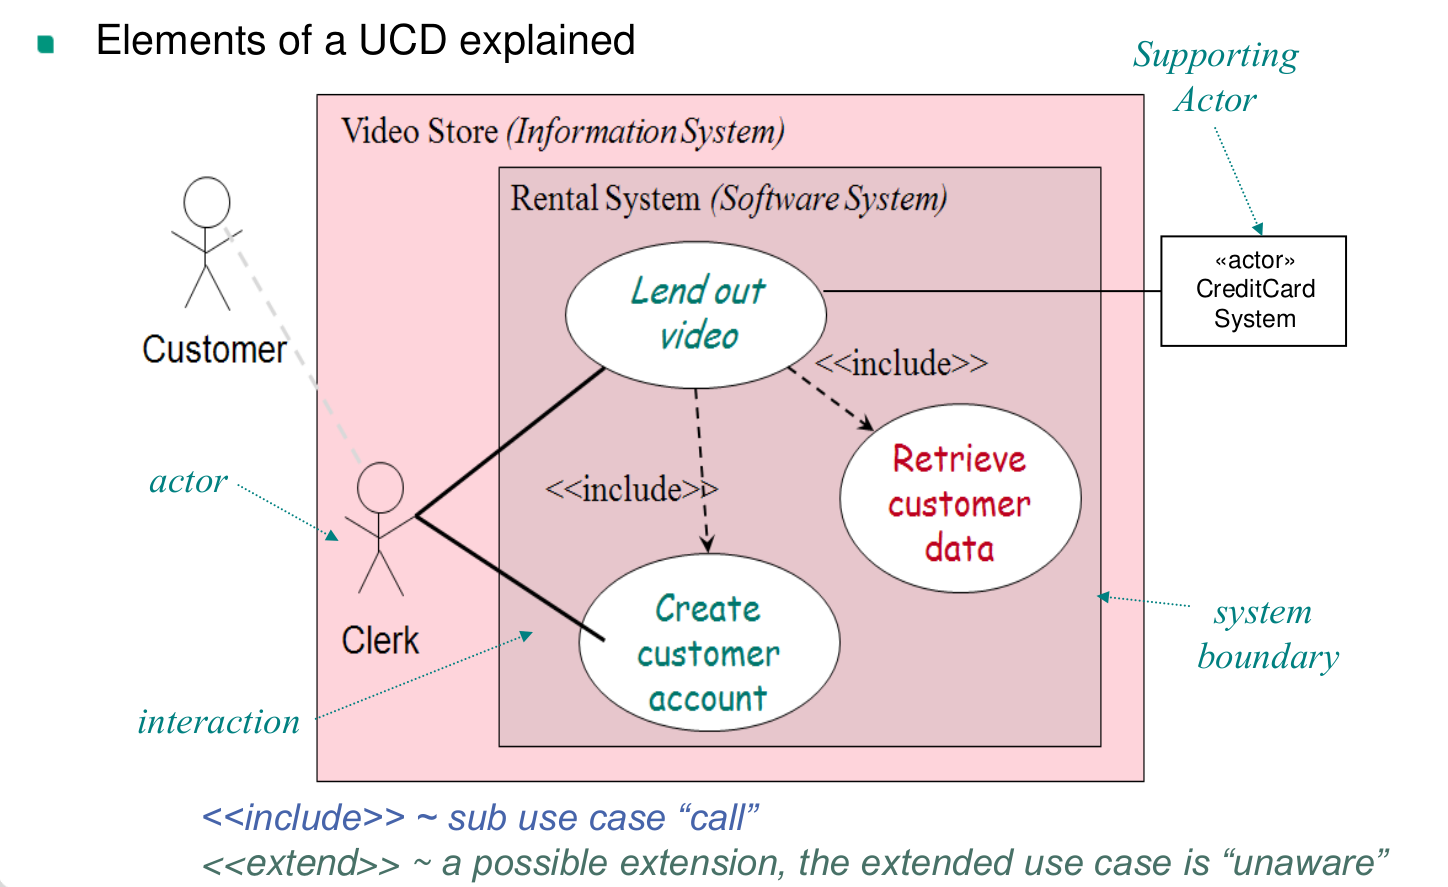
\includegraphics[width=0.85\textwidth]{images/usecase.png}
\end{figure}
	\section{Analysis}
\label{an:sec:analysis}

	\section{Software Design}
\label{sd:sec:software_design}

\subsection{Responsibility-Driven Design}
\label{sd:sub:responsibility_driven_design}

\begin{itemize}
	\item Betrachte \textbf{Responsibilities} der Softwareobjekte
	\item Unterteilung in \textbf{Doing Responsibilities} (was tut das Objekt?) und \textbf{Knowing Responsibilities} (was weiß das Objekt?)
	\item \textbf{Zuweisung von Responsibilities} beginnt oft bei \textbf{Operation Contracts}
	\item \textbf{Agile Methoden} arbeiten Responsibilities iterativ und informell aus, z.B auf Whiteboards mit \textbf{Interaktionsdiagrammen}
	\item \textbf{Design Class Diagrams (DCDs)} illustrieren u.a. Klassen, Assoziationen, Attribute, Interfaces, Methoden, Dependencies
\end{itemize}

\subsection{GRASP}
\label{sd:sub:grasp}

\textbf{G}eneral \textbf{R}esponsibility \textbf{A}ssignment \textbf{S}oftware \textbf{P}atterns

\begin{enumerate}
	\item \textbf{Information Expert}: Die Klasse, welche \textbf{alle notwendigen Informationen hat}, hat die Verantwortung
	\item \textbf{Creator}: Die Klasse, welche das Objekt \textbf{erstellt}, \textbf{erstellen kann} oder es \textbf{hauptsächlich nutzt}, hat die Verantwortung
	\item \textbf{Controller}: Ein \textbf{dedizierter Controller} (oder ein Fassaden-Objekt) hat die Verantwortung für (System)Events
	\item \textbf{Low Coupling}: Die Klasse mit den \textbf{wenigsten Dependencies} (lowest coupling) hat die Verantwortung
	\item \textbf{High Cohesion}: Die Klasse mit den \textbf{wenigsten verschiedenen Aufgaben} (highest cohesion) hat die Verantwortung
	\item \textbf{Polymorphism}: Statische \textbf{Factory-Methods} in der Base-Class haben die Verantwortung für die Erstellung von Objekten polymorpher Typen
	\item \textbf{Pure Fabrication}: Falls keine passende Klasse existiert, delegiere Verantwortung an eine \textbf{extra dafür hergestellte} Klasse um Coupling und Kohäsion zu erhalten
	\item \textbf{Indirection}: Delegiere Verantwortung für Kommunikation zwischen Klassen an \textbf{Adapter-Klassen}
	\item \textbf{Protected Variations}: Generelle Prinzipien zum Schutz vor Variationen (z.B \itquote{Don't talk to strangers})
\end{enumerate}
	\section{Architecture}
\label{arch:sec:architecture}

\begin{itemize}
	\item Resultat einer Menge von \textbf{Designentscheidungen}, welche die Struktur des Systems umfasst, darunter die \textbf{Komponenten}, ihre \textbf{Beziehungen} sowie ihr Mapping auf \textbf{Execution Environments}
	\item \textbf{View}: Repräsentation einer kohärenten Menge an Architekturelementen und ihrer Beziehungen aus der Sicht der Stakeholder (software architecture documentation)
	\item \textbf{Structure}: Die eigentlichen Architekturelemente (software architecture)
	\item \textbf{View Point}: Gruppiert Views nach Concerns
	\item Jedes System hat eine Struktur und damit eine \textbf{Architektur}, aber nicht zwingend eine aus bewussten Entscheidungen einer \textbf{Architektur-Dokumentation}
	\item Explizite Architektur fördert \textbf{Kommunikation, Analyse, Wiederverwertbarkeit, Planungseffizienz, Sicherheit, Performanz und Wartbarkeit}
	\item Architektur ist auch wichtig bei \textbf{agilen Methoden!}
	\item Zum Aufbau einer Architektur können \textbf{Referenz-Architekturen} herangezogen werden
\end{itemize}

\subsection{UP Architectural Views}
\label{arch:sub:up_architectural_views}

\begin{center}
	\begin{tabular}{| c | c | c |}
		\hline
		\textbf{View} 		& \textbf{Beschreibung}																				& \textbf{Diagramme}\\\hline
		Logical 			& \makecell{Wichtigste Layer,\\Subsysteme, Klassen etc.}											& \makecell{Klassen-, Paket- und\\Interaktionsdiagramme}\\\hline
		Process 			& \makecell{Prozesse, Threads\\und deren Interaktionen}												& \makecell{Klassen- und Interaktionsdiagramme\\mit Thread-Notation}\\\hline
		Deployment 			& Deployment von Prozessen																			& Deployment-Diagramme\\\hline
		Data 				& \makecell{Persistente Daten/Datenbanken\\und ihre Interaktionen}									& Klassendiagramme\\\hline
		Security 			& n/a 																								& n/a\\\hline
		Implementation 		& \makecell{Beschreibung der Organisation von\\Deliverables und ihren Quellen (z.B Source Code)} 	& keine\\\hline
		Development 		& n/a 																								& n/a \\\hline
		Use Case 			& Wichtigste Use Cases																				& Use Cases\\
		\hline
	\end{tabular}
\end{center}

\subsection{RUP Architectural Views}
\label{arch:sub:rup_architectural_views}

Auch \textbf{4+1 Architectural Views}:

\begin{center}
	\begin{tabular}{| c | c | c |}
		\hline
		\textbf{View} 									& \textbf{Beschreibung} 															& \textbf{Diagramme}\\\hline
		Logical View									& \makecell{Funktionalitäten für\\den Endnutzer} 									& \makecell{Klassen-, Kommunikations-\\und Sequenzdiagramme}\\\hline
		\makecell{Development/\\Implementation View}	& \makecell{Perspektive des\\Programmierers} 										& Paketdiagramme\\\hline
		Process View									& \makecell{Dynamische Aspekte, z.B\\Performanz, Concurrency, Scalability} 			& Aktivitätsdiagramme\\\hline
		Physical View									& \makecell{Perspektive des System-Engineers,\\Topologie auf dem Physical Layer} 	& Deploymentdiagramme\\\hline
		Scenarios/Use Cases								& \makecell{Validierung des Architekturdesigns} 									& Use Cases\\
		\hline
	\end{tabular}
\end{center}

\subsection{Architectural Patterns}
\label{arch:sub:architectural_patterns}

\begin{itemize}
	\item \textbf{Layered Architecture}:
	\begin{itemize}
		\item Einteilung in \textbf{Schichten}, welche \textbf{nur mit direkt benachbarten Schichten} kommunizieren
		\item Reduziert Komplexität, vereinfacht Testen, Separation of Concerns
		\item Erhöht oft die Klassenzahl durch Fassaden oder Transferobjekte
	\end{itemize}
	\item \textbf{Separation of Concerns}:
	\begin{itemize}
		\item Bspw. Trennung von UI (View) und Logik (Model)
		\item Ermöglicht ggf. Austauschen oder Erweitern um neue Module
	\end{itemize}
	\item \textbf{Model-View-Controller}:
	\begin{itemize}
		\item Aufteilung in \textbf{Kontroll-Logik} (Controller), \textbf{UI} (View) und \textbf{restlicher Logik} (Model)
		\item Nützliche Anwendung von \textbf{Separation of Concerns}
	\end{itemize}
	\item \textbf{Observer}:
	\begin{itemize}
		\item Design-Pattern, welches häufig im Zusammenhang mit MVC auftritt
		\item Mache Klasse \textbf{observable}, benachrichtige bei Änderungen andere Klassen (\textbf{Observer}), die sich bei ersterer registriert haben
		\item Observable benötigt \textbf{kein Wissen} über die beobachtenden Klassen
	\end{itemize}
\end{itemize}
	\section{Enterprise Application Patterns}
\label{eap:sec:enterprise_application_patterns}

\subsection{Domain Logic Patterns}
\label{eap:sub:domain_logic_patterns}

\itquote{How to represent the business logic?}

\begin{itemize}
	\item \textbf{Transaction Script}:
	\begin{itemize}
		\item Organisiere Logik für jeden Transaktionstyp in einer Prozedur, visualisiere als Sequenzdiagramm
		\item \textbf{Vorteil}: Simple Prozeduren, einfache Handhabung von Data Sources und Transaction Boundaries
		\item \textbf{Nachteil}: Schlechte Skalierung für komplexe Logik, Duplikation
	\end{itemize}
	\item \textbf{Domain Model}:
	\begin{itemize}
		\item Nutze Domain Model (Objektorientierte Modellierung)
		\item \textbf{Vorteil}: Gut für komplexe Logik
		\item \textbf{Nachteil}: Schwer wenn kein Verständnis von OOP, Mapping zur Data Source ist komplexer
	\end{itemize}
	\item \textbf{Table Module}:
	\begin{itemize}
		\item Einzelne Klasse implementiert die Business Logic für eine Tabelle, erhält Zeile einer Datenbank
		\item \textbf{Vorteil}: Mapping auf die Data Source ist einfach, Logik wird separiert
		\item \textbf{Nachteil}: Schlecht für komplexe Logik, da keine Objektinstanzen
	\end{itemize}
	\item Table Module am geeignetsten bis zu einer gewissen Komplexität, danach Domain Model
\end{itemize}

\subsection{Data Source Architectural Patterns}
\label{eap:sub:data_source_architectural_patterns}

\itquote{How to separate domain logic and data source?}

\begin{itemize}
	\item \textbf{Record Set}:
	\begin{itemize}
		\item In-memory Objekt, welches von überall im System einfach generiert und manipuliert werden kann
		\item Sieht aus wie das Ergebnis einer SQL Query
	\end{itemize}
	\item \textbf{Table Data Gateway}:
	\begin{itemize}
		\item Einzelne Instanz, welche den Zugriff auf eine Datenbank regelt
		\item Funktioniert nicht gut mit Domain Model, dafür mit Transaction Scripts
	\end{itemize}
	\item \textbf{Active Record}:
	\begin{itemize}
		\item Kapselt eine Datenbankzeile und die Logik für den Zugriff auf diese
		\item Gut für simple Logik, Data Mapper (siehe unten) für komplexe Logik
	\end{itemize}
	\item \textbf{Row Data Gateway}:
	\begin{itemize}
		\item Table Data Gateway für eine einzelne Datenbankzeile
	\end{itemize}
	\item \textbf{Identity Map}:
	\begin{itemize}
		\item Map aller bisher geladenen Objekte, um wiederholtes Laden zu vermeiden
	\end{itemize}
	\item \textbf{Data Mapper}:
	\begin{itemize}
		\item Layer von Mappern, welche Datenbankzeilen und in-memory Objekte getrennt hält und die Vermittlung übernimmt
		\item Geeignet, wenn Datenbankschema und Objektmodell separat entwickelt werden, für komplexe Logik oder wenn ein Domain Model genutzt wird
	\end{itemize}
\end{itemize}

\subsection{Object-Relational Mapping Structural Patterns}
\label{eap:sub:object_relational_mapping_structural_patterns}

\itquote{How to map objects to relational databases?}

\begin{itemize}
	\item \textbf{Single Table Inheritance}:
	\begin{itemize}
		\item Repräsentiere Vererbungshierarchie als \textbf{Tabelle mit Spalten für alle möglichen Felder}
		\item \textbf{Vorteil}: Einfach, keine Joins nötig, Verschieben von Feldern in der Hierarchie lässt Datenbank unverändert
		\item \textbf{Nachteil}: Unbenutzte Felder macht Handhabung verwirrend, oft große Tabellen, nur ein Namespace für alle Felder
	\end{itemize}
	\item \textbf{Class Table Inheritance}:
	\begin{itemize}
		\item Repräsentiere Vererbungshierarchie \textbf{mit einer Tabelle für jede Klasse}
		\item \textbf{Vorteil}: Nur relevante Spalten, da Felder der Basisklassen nicht in Kindklassen dupliziert werden, gut implementierbar für bestehende Schemata
		\item \textbf{Nachteil}: Mehrere Tabellen (d.h. Joins nötig, Performanceprobleme), Refactoring erschwert, Basisklassen können Bottleneck werden
	\end{itemize}
	\item \textbf{Concrete Table Inheritance}:
	\begin{itemize}
		\item Repräsentiere Vererbungshierarchie \textbf{mit einer Tabelle für jede konkrete Klasse}
		\item \textbf{Konkret}: Klassen duplizieren Felder der Basisklassen, d.h. Kindtabelle hat alle Spalten der Elternklassen
		\item \textbf{Vorteil}: Keine nutzlosen Felder, keine Joins wenn man von konkreten Mappern liest
		\item \textbf{Nachteil}: Refactoring bleibt erschwert, Änderung eines Feldes der Basisklasse beeinflusst alle Subklassen-Tabellen
	\end{itemize}
\end{itemize}
	\section{Clean Architecture}
\label{ca:sec:clean_architecture}

	\section{Components}
\label{c:sec:components}

	\section{Cloud Architecture}
\label{cla:sec:cloud_architecture}

\begin{itemize}
	\item \textbf{5 essenzielle Charakteristika von Cloud Services}:
	\begin{enumerate}
		\item \textbf{Elastic Scalability}
		\item \textbf{On-demand Self-Service}
		\item \textbf{Ubiquitous Network Access}
		\item \textbf{Resource Pooling}
		\item \textbf{Measured Service}
	\end{enumerate}
	\item \textbf{Service Delivery Models}:
	\begin{itemize}
		\item \textbf{Software as a Service (SaaS)}: Web-Applikationen wie z.B Google Apps
		\item \textbf{Platform as a Service (Paas)}: Development-/Execution-Environments wie Windows Azure
		\item \textbf{Infrastructure as a Service (IaaS)}: Infrastruktur, z.B Storage-Solutions wie Google Drive
	\end{itemize}
	\item \textbf{Service Deployment Models}:
	\begin{itemize}
		\item \textbf{Private Cloud}: Organisationsinterne Cloud (z.B File-Server eines Unternehmens)
		\item \textbf{Public Cloud}: Organisationsübereifende Cloud (z.B Google Drive für Privatnutzer)
		\item \textbf{Hybrid Cloud}: Mischung aus private und public Cloud
	\end{itemize}
	\item \textbf{Single Tenant Architecture}: Jeder Nutzer erhält einen gleich großen Anteil an Ressourcen (Hardware, OS, Applikationen)
	\item \textbf{Multi Tenant Architecture}: Unterschiedliche Aufteilung der Gesamtressourcen für jeden Nutzer
\end{itemize}

\subsection{Virtualisierung}
\label{cla:sub:virtualisierung}

\begin{itemize}
	\item \textbf{Allgemein}: Bereitstellen einer logischen Abstraktion von physischen Ressourcen
	\item Beispiel: \textbf{Virtuelle Maschinen}
	\begin{itemize}
		\item Emuliere ein Computersystem innerhalb eines anderen Computersystems
		\item \textbf{Hypervisor}: Kontrolliert installierte virtuelle Maschinen und ihre Nutzung von echter Hardware
		\item \textbf{Partitionierung}: Mehrere Maschinen mit eigenen Betriebssystemen auf demselben Server
		\item \textbf{Isolation}: Virtuelle Maschinen beeinflussen sich nicht gegenseitig
	\end{itemize}
	\item \textbf{Vorteile}: Energie-Effizienz, Verfügbarkeit (leichte Migration), einfacheres Management, kaum Performance-Verlust
\end{itemize}

\subsection{Architecture Principles}
\label{cla:sub:architecture_principles}

\begin{itemize}
	\item \textbf{Decentralization}: Kein \textbf{Single Point of Failure}, vermindere Bottlenecks bei der Skalierung
	\item \textbf{Asynchrony}: Das System macht in jedem Fall Fortschritt
	\item \textbf{Autonomy}: Individuelle Komponenten können Entscheidungen basierend auf lokalen Informationen treffen
	\item \textbf{Local Responsibility}: Jede Komponente ist verantwortlich für ihre eigene Konsistenz
	\item \textbf{Controlled Concurrency}: Keine oder limitierte Concurrency Control ist benötigt
	\item \textbf{Failure Tolerant}: Fehlschlagende Komponenten sorgen nicht für Unterbrechungen
	\item \textbf{Controlled Parallelism}: Granulare Abstraktionen ermöglichen Parallelität für Robustheit und Performance
	\item \textbf{Building Blocks}: Kleine Komponenten, die den Service zusammensetzen
	\item \textbf{Symmetry}: Keine spezifische Konfiguration für jeden Knoten, symmetrischer Umfang an Funktionalität
	\item \textbf{Simplicity}: Das System sollte so simpel sein wie möglich, aber nicht simpler
\end{itemize}
	\section{Microservices}
\label{ms:sec:microservices}

\begin{itemize}
	\item \textbf{Architektur-Stil}, bei dem eine Applikation aus vielen \textbf{kleinen Services} zusammengestellt ist
	\item Laufen in \textbf{eigenen Prozessen} und kommunizieren möglichst \textbf{lightweight} (HTTP resource API, REST)
	\item \textbf{Dezentralisierung}, z.B separate Datenbanken
	\item Unabhängigkeit jedes Services bzgl. \textbf{Deployment}, \textbf{Skalierbarkeit}, \textbf{Programmiersprache} und \textbf{Entwicklerteam}
	\item Gegenstück: \textbf{Monolith}
	\item \textbf{Typische Patterns}:
	\begin{itemize}
		\item \textbf{Tolerant Reader}: Ignoriere unbekannte Elemente, mache so wenig Annahmen wie möglich für Robustheit
		\item \textbf{Consumer-Driven-Contracts}: Repräsentation aller Erwartungen der Nutzer
		\item \textbf{Design for Failure}: Erwarte, erkenne und repariere fehlschlagende Services
		\item \textbf{Evolutionary Design}: Ständige Erweiterung, Ersetzung und Aktualisierung des Codes
	\end{itemize}
	\item \textbf{Vorteile}:
	\begin{itemize}
		\item Fokus auf \textbf{Modularität}, gut für große Teams
		\item \textbf{Unabhängige Entwicklung}, gut für viele Teams
		\item \textbf{Diversität} von Technologie (Programmiersprachen, Frameworks, Datenbanksystemen etc.)
	\end{itemize}
	\item \textbf{Nachteile}:
	\begin{itemize}
		\item \textbf{Fehleranfälligkeit} bei Kommunikation der Services
		\item \textbf{Schwere Konsistenz-Maintainance}
		\item \textbf{Koordination} der Services ist anspruchsvoll, benötigt erfahrene Teams
	\end{itemize}
	\item Mit steigender Komplexität \textbf{holen Microservices Monolithen ein}
\end{itemize}
	\section{Model-Driven Development}
\label{mdd:sec:model_driven_development}

\begin{itemize}
	\item \textbf{Charakteristika eines Modells}:
	\begin{itemize}
		\item \textbf{Representation Feature}: Modelle sind Repräsentationen natürlicher oder künstlicher Originale
		\item \textbf{Reduction Feature}: Modelle erfassen nur relevante Aspekte
		\item \textbf{Pragmatic Feature}: Modelle sind ihren Originalen nicht per se eindeutig zugeordnet
	\end{itemize}
	\item Modelle die \quotestyle{vor dem Original} hergestellt wurden sind \textbf{präskriptiv}, das Original \textbf{instanziiert} das Modell
	\item \textbf{Self-descriptive Models}: Modelle, die sich selbst erklären (z.B ein Klassendiagramm, das die Struktur eines Klassendiagramms beschreibt)
	\item \textbf{Metamodel}: Modell zur Beschreibung von Modellierung, meist mit einer formalen Sprache beschrieben (\textbf{Object Constraint Language, OCL})
	\begin{itemize}
		\item \textbf{Abstract Syntax}: Abstrakte Beschreibung der Konstrukte, aus denen das Modell besteht, ihrer Relationen und Eigenschaften (\textit{Locomotive: [power:int]})
		\item \textbf{Concrete Syntax}: Konkrete Beschreibung eines von der abstrakten Syntax beschriebenen Modells\\(\textit{Locomotive: [power = 1840]})
		\item \textbf{Static Semantics}: Beschreibung der Modellierungsregeln und Restriktionen\\(\textit{context Locomotive inv: self.power $>=$ 0})
		\item \textbf{Dynamic Semantics}: Beschreibung der Bedeutung der genutzten Konstrukte, meist in Fließtext\\(\textit{Das Metamodell beschreibt...})
	\end{itemize}
\end{itemize}

\subsection{Model-Driven Software Development}
\label{mdd:sub:model_driven_software_development}

\begin{itemize}
	\item \textbf{Model-driven Engineering (MDE)}: Beschreibung in einer Modellierungssprache mit Generatoren (z.B Code-Generatoren)
	\item \textbf{Model-driven Software Development (MDD)}: Anwendung von MDE für Software-Entwicklung
	\item \textbf{Model-based}:
	\begin{itemize}
		\item Modelle sind manchmal \textbf{Secondary Artifacts}
		\item Modelle werden für \textbf{Kommunikation und Dokumentation} genutzt
		\item Manuelle Analyse und Evaluation
	\end{itemize}
	\item \textbf{Model-driven}:
	\begin{itemize}
		\item Modelle sind \textbf{Primary Artifacts}
		\item Modelle dürfen nicht ausgelassen werden, sind ein integraler Bestandteil des Systems
		\item Explizites Spezifizieren, Entwickeln, Versionieren etc. von Modellen
		\item Analyse durch \textbf{Model Transformations}
	\end{itemize}
	\item \textbf{Ziele}:
	\begin{itemize}
		\item \textbf{Plattform-Unabhängigkeit} und -Interoperabilität
		\item Schnellere Entwicklung besserer, wartbarer Software
		\item Einfachere Bewältigung von \textbf{Komplexität} und \textbf{technologischem Wandel}
		\item Wiederverwertbarkeit
		\item Optimalere \textbf{Separation of Concerns}
	\end{itemize}
	\item \textbf{Erwartete Vorteile}: Geringere Kosten, schnellere Entwicklung besserer Software
\end{itemize}

\subsection{Model-Driven Architecture}
\label{mdd:sub:model_driven_architecture}

\begin{itemize}
	\item \textbf{Model-driven Architecture (MDA)}: Standardisierter Prozess von MDD der \textit{Object Management Group}
	\item \textbf{Computation-Independent Model (CIM)}: Beschreibung von Requirements
	\item \textbf{Platform-Independent Model (PIM)}: Operationsbeschreibungen ohne Implementationsdetails der Plattform
	\item \textbf{Platform-Specific Model (PSM)}: PIM mit zusätzlichem Fokus auf plattformspezifische Aspekte
\end{itemize}

\subsection{Model Transformations}
\label{mdd:sub:model_transformations}

\begin{itemize}
	\item \textbf{Transformation}: Automatische Generierung eines Zielmodells aus einem Quellmodell (z.B Code aus UML)
	\item \textbf{Transformationsdefinition}: Beschreibung des Transformationsprozesses von einem Modell ins andere
	\item \textbf{Transformationsregel}: Beschreibung des Transformationsprozesses eines einzelnen Konstruktes
\end{itemize}
	\section{Real-Time Design Patterns}
\label{rtdp:sec:real_time_design_patterns}

\begin{itemize}
	\item \textbf{Echtzeitsysteme / Real-time systems}:
	\begin{itemize}
		\item Systeme die ihre Umgebung beobachten und kontrollieren, oft \textbf{Embedded Systems} wie Sensoren
		\item \textbf{Zeit} als kritischer Faktor neben logischer Korrektheit (vgl. Airbag-System)
		\item \textbf{Soft real-time systems} operieren bei Zeitfehlern schlechter
		\item \textbf{Hard real-time systems} operieren bei Zeitfehlern fehlerhaft
	\end{itemize}
	\item \textbf{(A)periodische Stimuli} ereignen sich in (un)vorhersehbaren Zeitintervallen
	\item \textbf{Interrupts} übergeben bei Bedarf schlagartig die Kontrolle an eine vordefinierte Routine
	\item \textbf{Periodic Processes} managen weiter in passenden Zeitintervallen zusätzlich die korrekte Operation
	\item \textbf{Monitoring Systems} führen eine Operation aus, wenn sich ein bestimmter Stimulus ereignet (z.B Airbags)
	\item \textbf{Control Systems} kontrollieren das Verhalten durchgehend (z.B automatische Temperaturregelung)
	\item \textbf{Dimensionen von Dependability}: Availability, Reliability, Security, Safety (und Resilience)
	\item \textbf{Design}:
	\begin{itemize}
		\item Aufteilung in \textbf{Sensor} (registriert Stimulus) und \textbf{Actuator} (reagiert auf den Stimulus)
		\item Jedes \textbf{Sensor-Actuator-Paar} sollte einen eigenen Prozess haben
		\item \textbf{Schnelles Switching} zwischen Paaren muss durch die Systemarchitektur ermöglicht werden, nutze spezielle \textbf{Echtzeit-Betriebssysteme} mit \textbf{wenig Overhead}
		\item Programmierung in \textbf{Assembly}, aber auch zunehmend in C
		\item \textbf{Hardware Co-Design} für bestmögliche Performance und Kontrolle
	\end{itemize}
	\item \textbf{Scheduling}: Prozess-Management noch wichtiger als sonst, viele Strategien sind möglich, welche als \textbf{statisch/dynamisch} sowie \textbf{preemptive und non preemptive} kategorisiert werden:
	\begin{itemize}
		\item First In First Out (dynamisch, non preemptive, keine Prioritäten)
		\item Fixed Priorities (dynamisch, statische Prioritäten)
		\item Earliest-Deadline-First (EDF) (dynamisch, dynamische Prioritäten)
		\item Time-Slice-Scheduling (dynamisch, preemptive, keine Prioritäten)
		\item \textbf{Least-Laxity-First} (LLF, dynamisch, dynamische Prioritäten)
		\begin{itemize}
			\item Es gilt: $laxity = deadline - now - remaining\ process\ time$
			\item Negative laxity bedeutet, dass der Task seine Deadline \textbf{nicht mehr erreichen kann}
		\end{itemize}
	\end{itemize}
\end{itemize}

\subsection{Design Patterns}
\label{rtdp:sub:design_patterns}

\begin{itemize}
	\item \textbf{Channel}:
	\begin{itemize}
		\item Abstraktes Rohr, welches Daten sequenziell transformiert
		\item Mehrere Channel verbessern Performance, Reliability und Safety
		\item \textbf{Homogeneous Redundancy / Switch to Backup}: Gebe einem Channel einen \textbf{Zweitchannel} mit einem \textbf{Sekundärsensor} als \textbf{Fallback}, sollte der erste Channel einen Fehler erkennen
		\item \textbf{Triple Modular Redundancy}: Verarbeitung desselben Sensorwertes mit drei Channeln, Vergleich der Ergebnisse prüft auf Random Faults
		\item \textbf{Heterogeneous Redundancy}: Vereinigt Vorteile der vorherigen Ansätze mit nur zwei Channeln; wie Hom. Red. mit zusätzlichem Ergebnisvergleich beider Channel
	\end{itemize}
	\item \textbf{Monitor-Actuator}:
	\begin{itemize}
		\item Spezialfall von Heterogeneous Redundancy
		\item Kontrolle des Actuator Channels durch einen Monitoring Channel mit Sensor, der den Actuator prüft
		\item Davon abgeleitete Verallgemeinerung: \textbf{Sanity Check Pattern}
	\end{itemize}
	\item \textbf{Watchdog}: Ähnlich zu Monitor-Actuator, Channel sendet regelmäßigen Heartbeat an den \textbf{Watchdog}, der \itquote{bellt wenn er nicht gestreichelt wird}; \textbf{sehr lightweight}
	\item \textbf{Safety Executive}:
	\begin{itemize}
		\item Actuation-Channel mit \textbf{Integritätscheck und Watchdog}, der ein Signal verarbeitet und an einen Actuator weitergibt
		\item \textbf{Fail-safe Processing Channel}, der ebenfalls ein Signal erhält und an einen anderen Actuator weitergibt
		\item \textbf{Monitor} beobachtet beide Channel, \textbf{kann beide Channel abschalten}, falls der Actuation-Channel fehlschlägt oder den Watchdog alarmiert
	\end{itemize}
\end{itemize}
	\section{Security}
\label{sc:sec:security}

\begin{itemize}
	\item \textbf{Ziele}: Verfügbarkeit, Vertraulichkeit und Integrität von Daten und System
	\item \textbf{Weitere Ziele}: Nutzer-Authentifizierung, Verfolgbarkeit, Anonymität
	\item Sicherheitslücken entstehen oft durch \textbf{Zeitmangel, Geldmangel, Erfahrungsmangel der Entwickler} oder anderem \textbf{Einsatz-Kontext}
	\item \textbf{Technische Gründe}: Nutzung von Pseudo-Zufall, Race Conditions, fehlende Input-Validierung (Overflows)
	\item Security muss \textbf{früh beachtet werden}; präventives \textbf{Penetration Testing (pentesting)}
	\item Security-Management at run-time: \textbf{Resilience}
\end{itemize}

\subsection{Principles for Building Secure Software}
\label{sc:sub:principles_for_building_secure_software}

\begin{enumerate}
	\item \textbf{Secure the weakest link}: selbsterklärend; beachte: weakest link ist nicht zwingend Software (social engineering)
	\item \textbf{Practice defence in depth}: Mehrere Schutzschichten
	\item \textbf{Fail securely}: Keine Exposure von Systemdetails bei Fehlschlag
	\item \textbf{Secure by default}: Aktiviere standardmäßig alle Sicherheitsfeatures
	\item \textbf{Principle of least privilege}: Jeder erhält nur minimale nötige Privilegien
	\item \textbf{No security through obscurity}: Keine versteckten magic URLs, Logins, Cheats o.ä. (reverse engineering möglich)
	\item \textbf{Minimize attack surface}: Weniger Code reduziert Angriffsfläche
	\item \textbf{Privileged Core}: Isolierter Kern mit Sicherheits-Privilegien
	\item \textbf{Input Validation and Output Encoding}: Nur valide Inputs erlauben, Outputs sollten nicht ausführbar sein
	\item \textbf{Don't Mix Data and Code}: Overflows vermeiden, Daten externalisieren (z.B Passwörter)
\end{enumerate}

\subsection{Weitere Sicherheitsmaßnahmen}
\label{sc:sub:weitere_sicherheitsmassnahmen}

\begin{itemize}
	\item \textbf{Federated Identity Management} (z.B LDAP), nicht das Rad neu erfinden
	\item Starke \textbf{Passwörter}, niemals im Client auswerten, stattdessen auf dem Server hashen und auswerten
	\item \textbf{Session Handling} in Web-Apps
	\item Fokus auf Dokumentation
	\item Lerne \textbf{Schwächen der genutzten Software} und \textbf{Programmiersprachen}
	\item \textbf{Code Coverage Tools}
	\item \textbf{Externe Evaluation}, Sicherheitszertifikate
	\item Korrektes Handling von \textbf{Threads}: Atomare Operationen nutzen, Critical Sections, Semaphoren etc.
\end{itemize}
	\section{Bonus: Vortrag von Andrena Objects}
\label{bn:sec:bonus_vortrag_von_andrena_objects}

\end{document}
